\section{Feature Extraction}
In this section it will be explained how the original MNIST dataset have been processed to create a feature set other than the raw pixel values. First the original data is outlined.
\subsection{MNIST Dataset}
The MNIST Dataset consist of 60000 examples of handwritten digits for training and 10000 for testing. It will be shown later how pixels in such images are highly correlated and the real dimension of the data is much lower using PCA analysis.


\begin{figure}[hbtp]
\centering
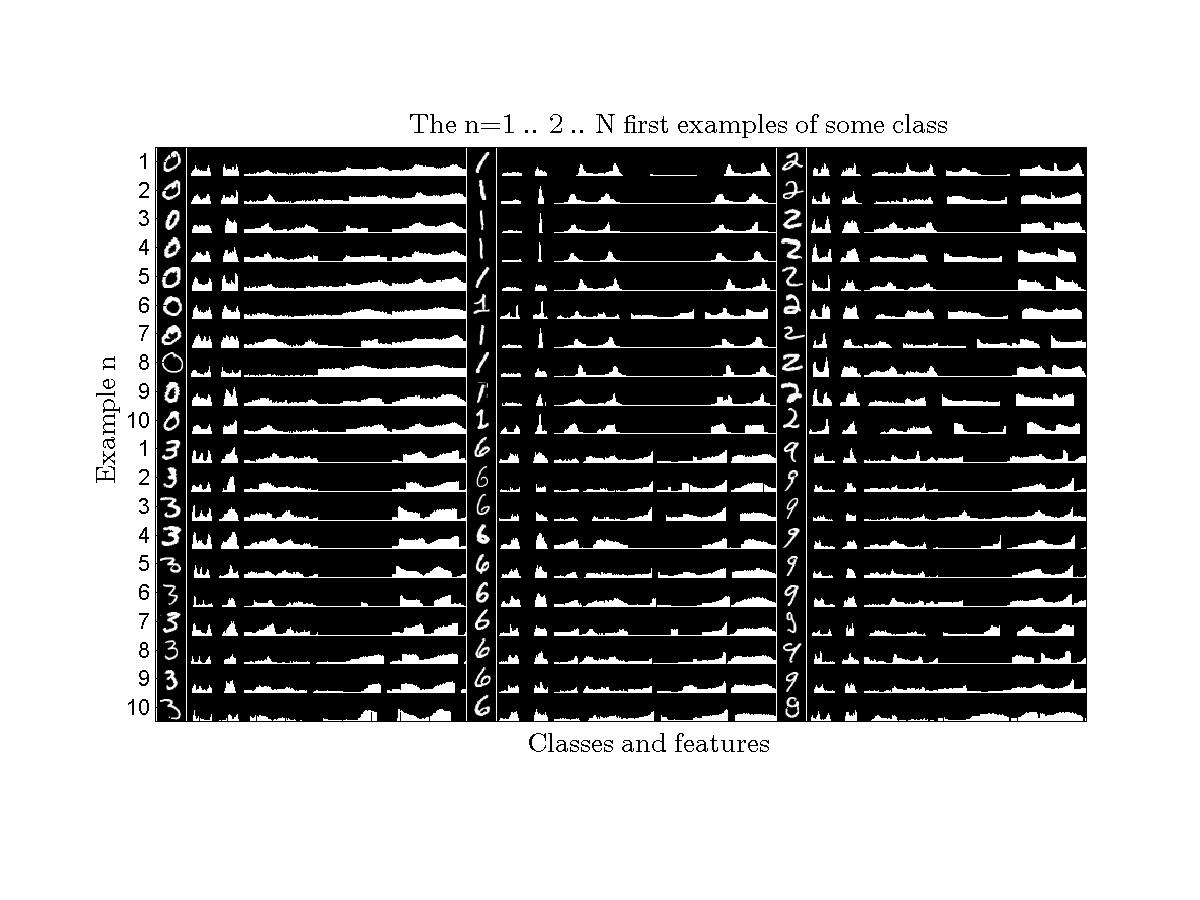
\includegraphics[width=\linewidth]{feature_examples}
\caption{10 Examples of six classes in the dataset and the extracted features. Features consist first of vertical[28], horizontal[28] and radial[72] histograms and in-out[72], out-in[72] profiles to a total of 272 features. \label{fig:image_examples}}
\end{figure}

In Figure~\ref{fig:image_examples} ten examples of six picked classes are shown and a lot of variance can be seen for each individual class when looking at the image and some patterns may be detected in the extracted features. The goal is then to get the machine learning algorithm to find the patterns and separate them based on the label information.
\subsection{Extraction}
Feature extraction have been done by computing Structural Characteristics of each 28 by 28 pixel image from MNIST as outlined in \cite{1227727}. This process extracts a vertical, horizontal and radial histogram concatenated with an in-out and out-in profile.

In Figure~\ref{fig:image_examples} the features can be seen next to its input image. The radial histogram and profiles are computed as 72 steps of 5 degrees. The profiles are the distance to the first and last on-pixel from the center and out. 

This means that all of our attributes are discrete and ratio, since the absence of value in an attributes actually means that there are no pixels in the set of pixels, and the fact that the distance between attribute values are comparable by factors (ratio).
